\section{Computation of the error}

Solving PDEs numerically will result in errors because derivatives are approximated by finite differences and the PDE is required to be fulfilled only on the mesh points. 
% For the schemes used in this thesis the error, $\epsilon$ will follow equation \eqref{analysis:error}
% 
% \begin{equation}\label{analysis:error}
%  \epsilon = C_x\Delta x^2 + C_t\Delta t
% \end{equation}
% 
% \noindent where the coefficients $C_x$ and $C_t$ are unknown. 
% Notice that there is one term arising from the time derivative and one from the spatial derivative and that they are of different order. 

The error, $\epsilon$, is measured by comparing the result from a numerical simulation to an exact solution, $u_e$ and taking the norm of the difference. 
Specifically $\epsilon$ is measured by the L2 norm which is defined in \eqref{analysis:def_epsilon}:
% \label{analysis:def_epsilon}
\begin{align}
 \epsilon(t^k) &= ||u(t^k)-u_e(t^k)||_2 \nonumber \\
 &= \iint\sqrt{\left(u(t^k,x,y)-u_e(t^k,x,y)\right)^2}\,dx\,dy \nonumber \\
 &\approx \sqrt{\Delta x\Delta y\sum\limits_{i=0}^k\sum\limits_{i=0}^k \left(u(t^k,x_i,y_j)-u_e(t^k,x_i,y_j)\right)^2}.\label{analysis:def_epsilon}
 \end{align}
 
\noindent A time dependent error estimate has been chosen because it allows for investigation of the evolution of the error over the course of a simulation.
Some of the error tests will require a single number as an error measure. 
In these cases the norm of $\epsilon(t)$, shown below, is used:
\begin{equation}\label{analysis:convergence_test_error}
 \epsilon = \sqrt{\Delta t\sum\limits_{k=0}^T\epsilon(t^k)^2}.
\end{equation}

\section{Verification techniques}
All parts of the hybrid diffusion solver are subject to testing. First, the PDE and RW solver will be tested individually, then the hybrid solver is tested. 
This thesis will focus on three verification techniques which are described below. 
The aim for all of these techniques is to make sure that the implementation is correct by comparing simulations to an exact solution. \\

\noindent For the PDE solver, there are errors arising from both the spatial derivative and from the time derivative. 
Since an incorrect implementation of the spatial derivative will cause the solution to be unstable, which is easily noticed through visual inspection, the tests will focus on verifying the time derivative. 
In some cases, isolating the contribution to $\epsilon(t)$ from the time derivative will be necessary, and is ensured by setting $\Delta t \gg\Delta x^2$. 
A time step of this size violates the stability criterion for the FE scheme, and so some of the tests are slightly inaccurate for this scheme. \\

The verification techniques that will be carried out are:

\begin{itemize}
 \item Manufactured solutions\\
 By adjusting the source term, $s(x,t)$, one can, in principle, choose any solution to the diffusion equation. 
Should we, for example, want the solution to be $u(x,t) = \frac{1}{x+1}$, all that is needed is to set the source term equal to $-D\frac{\d^2 u}{\d x^2}$;
\begin{equation*}
s(x,t) = \frac{2D}{(x+1)^3},
\end{equation*}
and the problem is solved (as long as the boundary conditions are correct).
 For the verifiation that follows, the chosen solution is
 \begin{equation}\label{manufactured_solution}
  u(x,y,t) = e^{-\pi^2t}\cos(\pi x)\cos(\pi y) +1,
 \end{equation}
 which requires no source term and fulfills the zero flux boundary conditions naturally. 
  The point of these tests is to verify that $\epsilon \sim \Delta t$ and the tests can be done for a time step which fulfills the stability criterion.
  \item Convergence tests \\
%   In the general case the error term is proportional to the time step to some power $r$ when the error from the time derivative is dominant.
 For the schemes used in this thesis the error term is described by
\begin{equation}\label{analysis:error}
 \epsilon = C_x\Delta x^2 + C_t\Delta t^1,
\end{equation}
where the coefficients $C_x$ and $C_t$ are unknown. 
Notice that there is one term arising from the time derivative and one from the spatial derivative and that they are of different order. \\
Where possible, convergence will be tested by isolating one of the error terms. For example, setting $\Delta t \gg \Delta x^2$, implies $C_x\Delta x^2\approx0$ and 
$$
\epsilon \propto \Delta t^r,
$$
where $r=1$. 
As $\Delta t$ tends to zero, $r$ is expected to converge to one, and that is the purpose of these tests. 
By comparing the error from two simulations with different time steps, the convergence rate, $r$, can be measured from 
 \begin{align*}
   r&\simeq \frac{\log\left(\epsilon_1/\epsilon_2\right)}{\log\left(\Delta t_1/\Delta t_2\right)}.
\end{align*}
Notice that a single number must be used to describe the error, as shown in \eqref{analysis:convergence_test_error}.

  \item Exact numerical solutions \\
  The numerical schemes are actually reformulations of the PDE as difference equations, which have their own exact solutions. 
  These will be called the numerical exact solutions, and they are slightly different from the exact solutions to the PDE. 
  The reason for finding the numerical exact solutions is that the scheme theoretically will represent this solution with no error. 
  In practice there will always be round off errors and other factors, but an error term close to machine precision is expected.
\end{itemize}

\section{Testing the PDE solver}


\subsection{Verification by manufactured solutions}\label{analysis:section_manufactured_solution}

Equation \eqref{manufactured_solution} solves the diffusion equation, so using $u(x,y,t=0)$ as the initial condition for a simulation will give us both the numerical solution and the exact solution. 
An important property of both the FE and BE discretization schemes is that the difference between these solutions is of the same order as the time step.
\begin{equation*}
 \epsilon(t) \sim \mathcal{O}(\Delta t)
\end{equation*}
% \noindent For the FE scheme a single discretization parameter will be introduced by having a constant relation between the spatial resolution and the time step 
% \begin{equation*}
%  \frac{\Delta t}{\Delta x^2} = k
% \end{equation*}
% $\epsilon(t)$ can now be rewritten by setting $\Delta t = h$
% \begin{align*}
%  \epsilon(t) &= C_t h + C_x\frac{h}{k} \\
%  &= (C_t +C_x/k)h = C_k h
% \end{align*}

Figures \ref{analysis:errorplots:FE} and \ref{analysis:errorplots:BE} show that for both the FE and BE scheme in both 1D and 2D the error is of the expected magnitude, which is roughly $\Delta t$. 
Another interesting property of the error plots is that the error tends to zero after a large number of time steps. 
By inserting the limit $t\to\infty$ in \eqref{manufactured_solution} we observe that the error is expected to tend to zero because the limit value of one can be exactly recreated by both schemes.
\begin{align*}
 \lim_{t\to\infty} e^{-\pi^2t}\cos(\pi x)\cos(\pi y) +1 = 1
\end{align*}

\begin{figure}[H]
% Error plots for FE in 1D (a) and 2D (b)
 \centering
 \begin{subfigure}{0.49\textwidth}
  \includegraphics[width=\textwidth]{../results/experiment_22052014_1327_FE1D_new_plots/results/errorplot_pretty.eps}
  \caption{}
  % experiment_22052014_1305_spatial_convergencetest_BE1D
 \end{subfigure}
 \begin{subfigure}{0.49\textwidth}
  \includegraphics[width=\textwidth]{../results/experiment_22052014_1323_FE2D_new_plots/results/errorplot_pretty.eps}
  \caption{}
% experiment_22052014_1309_spatial_convergencetest_BE1D
 \end{subfigure}
 \caption[Error plots FE]{Error plot for the FE scheme in 1D (a) and 2D (b). All simulations have been run using $\Delta t = \frac{\Delta x^2}{5}$ which fulfills the stability criterion in 1D and 2D.}
 \label{analysis:errorplots:FE}
\end{figure}


\begin{figure}[H]
% Error plots for BE in 1D (a) and 2D (b)
\centering
 \begin{subfigure}{0.49\textwidth}
  \includegraphics[width=\textwidth]{../results/experiment_14052014_0744_errorplot_BE1D/results/errorplot_pretty.eps}
  \caption{}
 \end{subfigure}
 \begin{subfigure}{0.49\textwidth}
  \includegraphics[width=\textwidth]{../results/experiment_22052014_1317_BE2D_new_plots/results/errorplot_pretty.eps}
  \caption{}
 \end{subfigure}
 \caption[Error plots BE]{Error plot for the BE scheme in 1D (a) and 2D (b). Notice that the error is roughly of the same order as the time step. Figures \ref{analysis:errorplots:FE}b and \ref{analysis:errorplots:BE}b show the same simulation using FE and BE schemes in 2D. The error is slightly larger in the BE discretization by a factor of 4.}
 \label{analysis:errorplots:BE}
\end{figure}

\subsection{Verification by convergence tests}

The convergence tests are done by isolating the error term from either the time derivative or the spatial derivative, and refining the relevant discretization parameter over several simulations. 
However, for the FE scheme it is impossible to isolate the error from the time derivative without violating the stability criterion. 
To cope with this problem a single discretization parameter, $h$, is introduced by ensuring  
\begin{equation*}
 \frac{\Delta t}{\Delta x^2} = k,
\end{equation*}
where $k$ is a constant. 
The error term from \eqref{analysis:error} can now be rewritten by setting $\Delta t = h$;
\begin{align*}
 \epsilon(t) &= C_t h + C_x\frac{h}{k} \\
 &= (C_t +C_x/k)h \\
 &= C_k h^r,
\end{align*}
where $r$ is still expected to converge to one.  \\

\noindent Figures \ref{analysis:convergence_tests:FE} and \ref{analysis:convergence_tests:BE} verify that the error associated with the time derivative is of the expected order. 

In Figure \ref{analysis:spatial_convergence_tests} the error from the spatial derivative has been isolated, and tested for both schemes. 
The error term associated with the spatial derivative is of second order, as seen in \eqref{analysis:error}. A second order error term is expected to have second order convergence.

\begin{figure}[h]
% Convergence tests for FE in 1D (a) and 2D (b)
\centering
 \begin{subfigure}{0.49\textwidth}
  \includegraphics[width=\textwidth]{../results/experiment_18042014_1014_convergencetest_FE1D/results/ConvergenceTest.eps}
  \caption{}
 \end{subfigure}
 \begin{subfigure}{0.49\textwidth}
  \includegraphics[width=\textwidth]{../results/experiment_27052014_1152_FE2D_new_convergence_time/results/ConvergenceTest_pretty.eps}
  \caption{}
 \end{subfigure}
 \caption[Convergence tests in time FE scheme]{Convergence tests with respect to the single discretization parameter, $h$, for the FE scheme in 1D (a) and 2D (b). }
 \label{analysis:convergence_tests:FE}
\end{figure}

\begin{figure}[h]
% Convergence tests for BE in 1D (a) and 2D (b)
\centering
 \begin{subfigure}{0.49\textwidth}
  \includegraphics[width=\textwidth]{../results/experiment_14052014_0744_errorplot_BE1D/results/ConvergenceTest.eps}
  \caption{}
 \end{subfigure}
 \begin{subfigure}{0.49\textwidth}
  \includegraphics[width=\textwidth]{../results/experiment_18042014_1450_convergencetest_BE2D/results/ConvergenceTest.eps}
  \caption{}
 \end{subfigure}
 \caption[Convergence tests for BE scheme]{Convergence tests with respect to the time derivative for the BE scheme in 1D (a) and 2D (b).}
 \label{analysis:convergence_tests:BE}
\end{figure}

\begin{figure}[H]
% Spatial error tests 
\centering
 \begin{subfigure}{0.49\textwidth}
  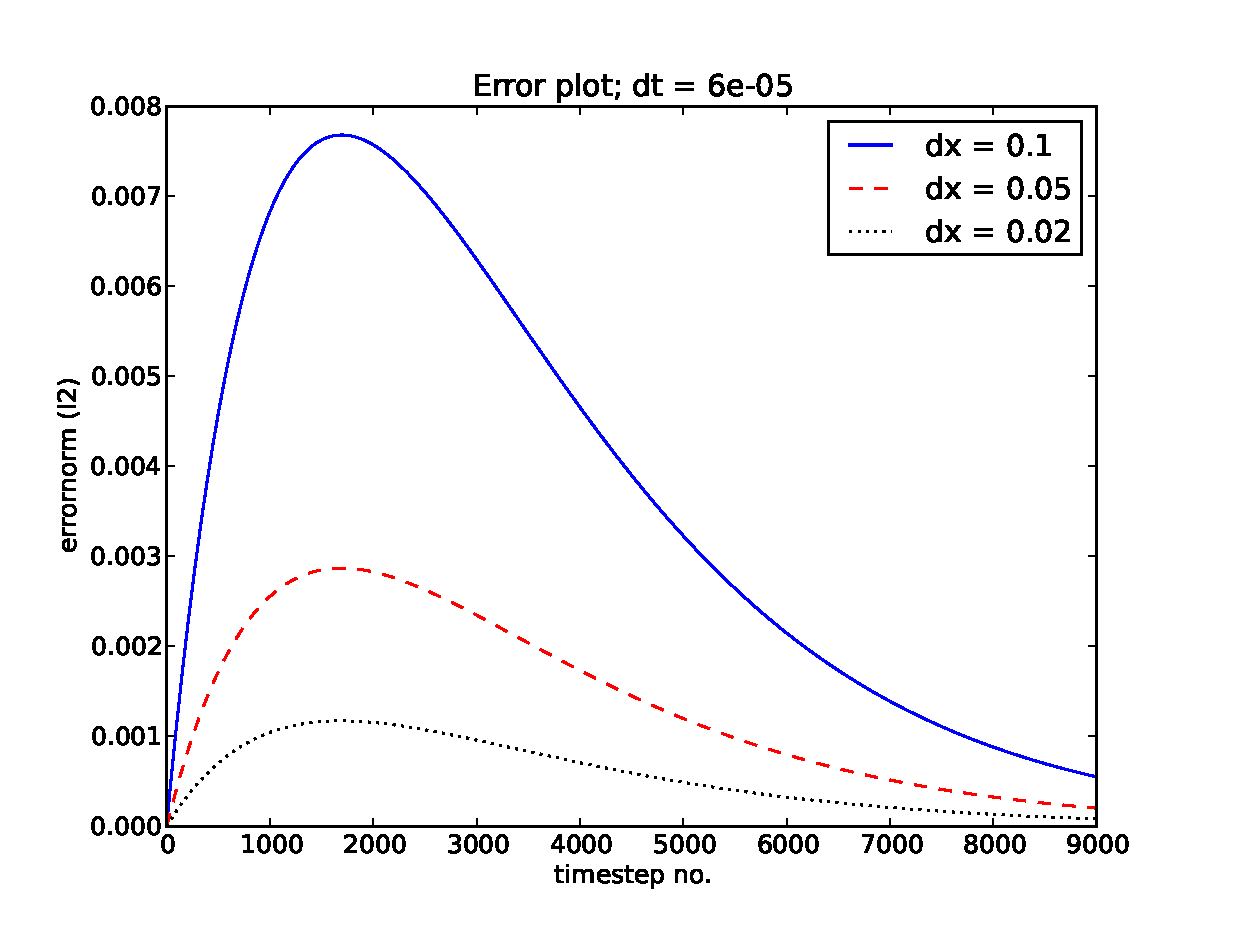
\includegraphics[width=\textwidth]{../results/experiment_22052014_1254_spatial_convergencetest_BE1D/results/errorplot.eps}
  \caption{}
 \end{subfigure}
 \begin{subfigure}{0.49\textwidth}
  \includegraphics[width=\textwidth]{../results/experiment_22052014_1254_spatial_convergencetest_BE1D/results/ConvergenceTest.eps}
  \caption{}
 \end{subfigure}
 
  \begin{subfigure}{0.49\textwidth}
  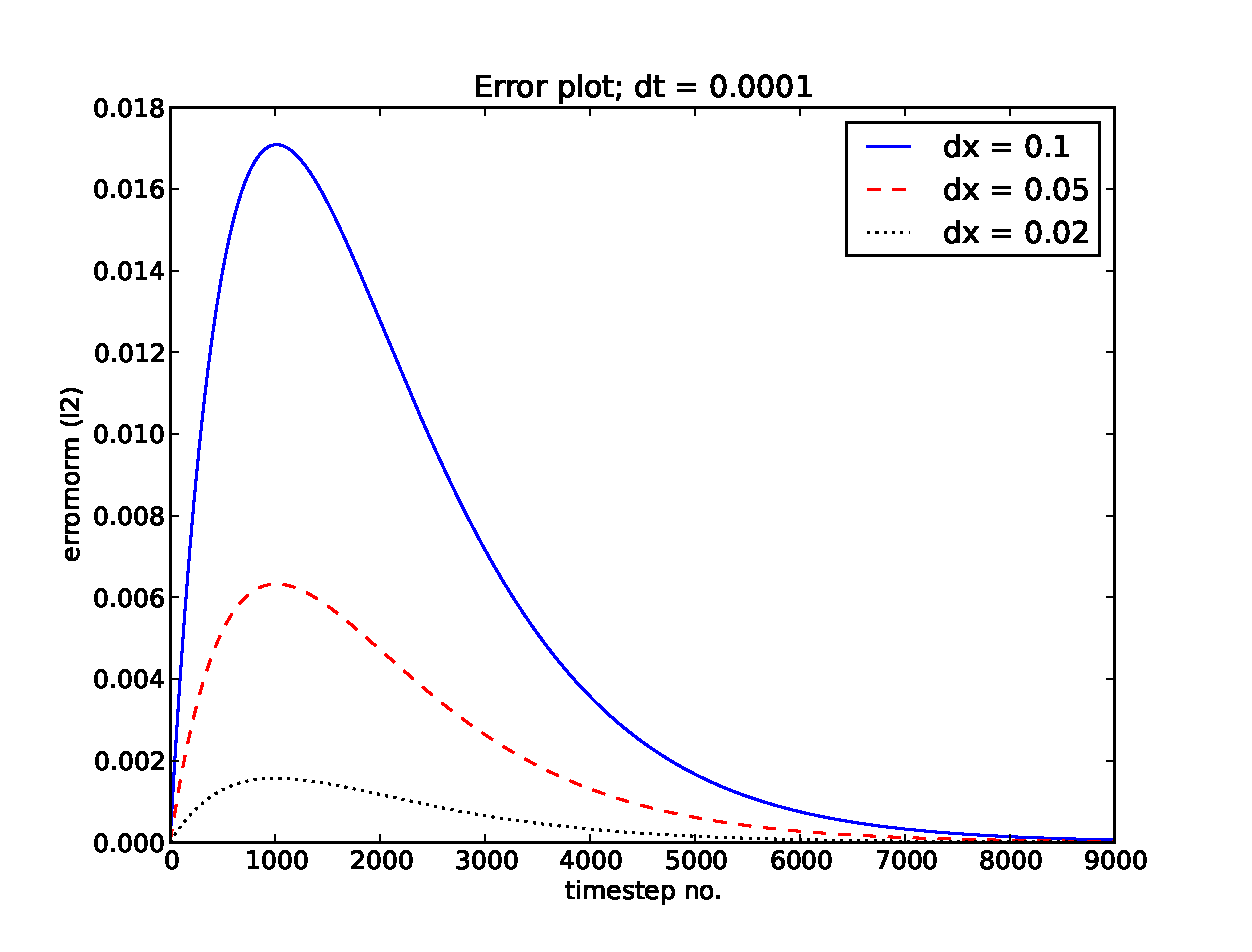
\includegraphics[width=\textwidth]{../results/experiment_22052014_0810_spatial_convergencetest_FE2D/results/errorplot.eps}
  \caption{}
 \end{subfigure}
 \begin{subfigure}{0.49\textwidth}
  \includegraphics[width=\textwidth]{../results/experiment_22052014_0810_spatial_convergencetest_FE2D/results/ConvergenceTest.eps}
  \caption{}
 \end{subfigure}
 \caption[Spatial error tests]{These plots show the error and convergence from the spatial derivative using BE (a \& b) and FE (c \& d) discretization schemes. The expected convergence rate for both discretizations is $r = 2$, which is recreated to a decent accuracy. Testing has been done using 1D simulations for the BE scheme, and 2D simulations for the FE scheme. This should not make any difference for the results.}
 \label{analysis:spatial_convergence_tests}
\end{figure}


\subsection{Verification of FE scheme by exact numerical solution}\label{exact_numerical_solution}

Discretization of the diffusion equation by the FE scheme yields the following numerical scheme in 1D:
\begin{equation}\label{analysis:simplified_FE_scheme}
 u^{k+1} = D\Delta t u^k_{xx} + u^k,
\end{equation}
where $u_{xx}$ denotes the double derivative of $u$ with respect to $x$. 
\eqref{analysis:simplified_FE_scheme} is a difference equation, which is most easily solved by writing out the first four iterations and finding a pattern
% To illustrate how the equation is solved by the computer, the first four iterations are written out
\begin{align*}
 u^1 &= D\Delta t\, u_{xx}^0 + u^0 \\
 u^2 &= D\Delta t\, u_{xx}^1 + u^1 \\
 &= D\Delta t\left[D\Delta t u_{4x}^0 + u_{2x}^0\right] + D\Delta t\, u_{xx}^0 +u^0\\
 &= \left(D\Delta t\right)^2 u_{4x}^0 + 2D\Delta t u_{2x}^0+ u^0 \\
 u^3 &= D\Delta t\, u_{xx}^2 + u^2 \\
 &= D\Delta t\left[\left(D\Delta t\right)^2 u_{6x}^0 + 2D\Delta t u_{4x}^0+ u_{2x}^0\right] + \left(D\Delta t\right)^2 u_{4x}^0 + 2D\Delta t u_{2x}^0+ u^0\\
 &= \left(D\Delta t\right)^3 u_{6x}^0 + 3\left(D\Delta t\right)^2 u_{4x}^0+ 3D\Delta tu_{2x}^0 + u^0 \\
 u^4 &= D\Delta t \,u_{xx}^3 + u^3 = \dots \\
 &= \left(D\Delta t\right)^4 u_{8x}^0 + 4\left(D\Delta t\right)^3 u_{6x}^0+ 6\left(D\Delta t\right)^2 u_{4x}^0 + 4D\Delta t u_{2x}^0 + u^0 
\end{align*}

\noindent From the iterations above a pattern can be recognized for iteration $k+1$:\\
\begin{equation}
 u^{k+1} = \sum\limits_{i=0}^k {k\choose i}\left(D\Delta t\right)^iu^0_{2ix},
\end{equation}
where $u^0$ is the initial condition;
\begin{equation}
 u^0 = \cos(\pi x).
\end{equation}
The spatial derivatives are found by inserting the initial condition into the centered difference approximation to the second derivative :
\begin{align*}
 u^0_{xx} &= \frac{1}{\Delta x^2}\left(\cos(\pi(x+\Delta x)) -2\cos(\pi x) +\cos(\pi(x-\Delta x))\right) \\
 &= \frac{2}{\Delta x^2}\left(\cos(\pi\Delta x)-1\right)\cos(\pi x)\\
 u^0_{4x} &= [u^0_{xx}]_{xx} \frac{1}{\Delta x^2}\left[\frac{u^0_{xx}}{\cos(\pi x)}\left(\cos(\pi(x+\Delta x)) -2\cos(\pi x) +\cos(\pi(x-\Delta x))\right)\right]\\
 &= \frac{4}{\Delta x^4}\left(\cos(\pi\Delta x)-1\right)^2\cos(\pi x)\\
 &\dots
\end{align*}
The pattern continues allowing the final numerical exact solution to be expressed below:
\begin{equation}\label{numerical_solution}
  u^{k+1} = \sum\limits_{i=0}^k {k\choose i}\left(D\Delta t\right)^i\frac{2^i}{\Delta x^{2i}}\left(\cos(\pi\Delta x)-1\right)^i\cos(\pi x).
\end{equation}
By construction the Neumann boundary conditions are fulfilled since $\frac{\d \cos(\pi x)}{\d x} = -\pi\sin(\pi x)$ and $\sin(0) = \sin(\pi) = 0$. \\

Although the FE scheme is expected to reproduce \eqref{numerical_solution} to machine precision ($\epsilon \approx 10^{-16}$) there are two problems with the solution which will have an effect on the error:
\begin{itemize}
 \item $\Delta x^{2i}$ will quickly tend to zero, and the computer will interpret it as zero. This will cause division by zero, which again results in ``Not a number'' (nan) and ruins the simulation. Testing if $\Delta x^{2i}>0$ and returning zero if the test fails will fix the problem. The argumentation for ignoring the troublesome terms is given below.
 \item ${k\choose i}$ goes to infinity for large $k$ and $i$. The computer can only represent numbers up to $\sim10^{308}$, which limits the number of steps to $170$ since $k!>10^{308}$ for $k>170$.
\end{itemize}

As a side note, \eqref{numerical_solution} illustrates how the stability criterion for the FE scheme comes into place. 
In the numerical exact solution, the exponential which is found in the exact solution to the PDE (eq. \ref{manufactured_solution}) is replaced by an amplification factor $A^k$.
This amplification factor can be found in equation \eqref{numerical_solution} as 
\begin{equation}
A^k = \left(\frac{2D\Delta t}{\Delta x^2}\right)^i.
\end{equation}
Inserting a time step larger than $\frac{\Delta x^2}{2D}$ will make the amplification factor, $A$, larger than one, which in turn makes the solution blow up. \\

\noindent The stability criterion also illustrates why the terms where 
$$ \frac{1}{\Delta x^{2i}} \to \infty$$
 can be dropped. 
 By the stability criterion, the time step will cancel out $\Delta x^2$, and the result will be a number smaller than 1 raised to a rather large power, resulting in a number comparable to zero.\\
 
 The results from comparing a 1D simulation to the numerical exact is shown in Figure \ref{numerical_exact_FE:1D}. 
 As expected the error is larger than machine precision by at most two orders of magnitude because of accumulating error terms from the dropped terms in \eqref{numerical_solution}.\\
 
\noindent Using the same method as in the 1D case, a numerical exact solution can be found to the 2D FE scheme; 
 \begin{equation}\label{exact_numerical_solution_2d}
 u^{k+1} = \sum\limits^k_{i=0}{k\choose i}\left(D\Delta t\right)^i\left[2^{i-1}\cos(\pi x)\cos(\pi y)\left(\frac{(\cos(\pi\Delta x))^i}{\Delta x^{2i}} +\frac{(\cos(\pi\Delta y))^i}{\Delta y^{2i}}\right)\right].
\end{equation}

The same problems as in the 1D case will apply to \eqref{exact_numerical_solution_2d} with the same solutions. 
Figure \ref{numerical_exact_FE:2D} shows how the 2D simulation compares to the numerical exact solution. 
As was the case in 1D, the error is larger than machine precision, but much smaller than $\Delta t$.
% suggesting that the scheme is implemented correctly.

\begin{figure}[H]
 \centering
 \begin{subfigure}{0.49\textwidth}
 \includegraphics[width=\textwidth]{Figures/exact_numerical_1d_n130.eps}
  \caption{}
  \label{numerical_exact_FE:1D}
 \end{subfigure}
 \begin{subfigure}{0.49\textwidth}
 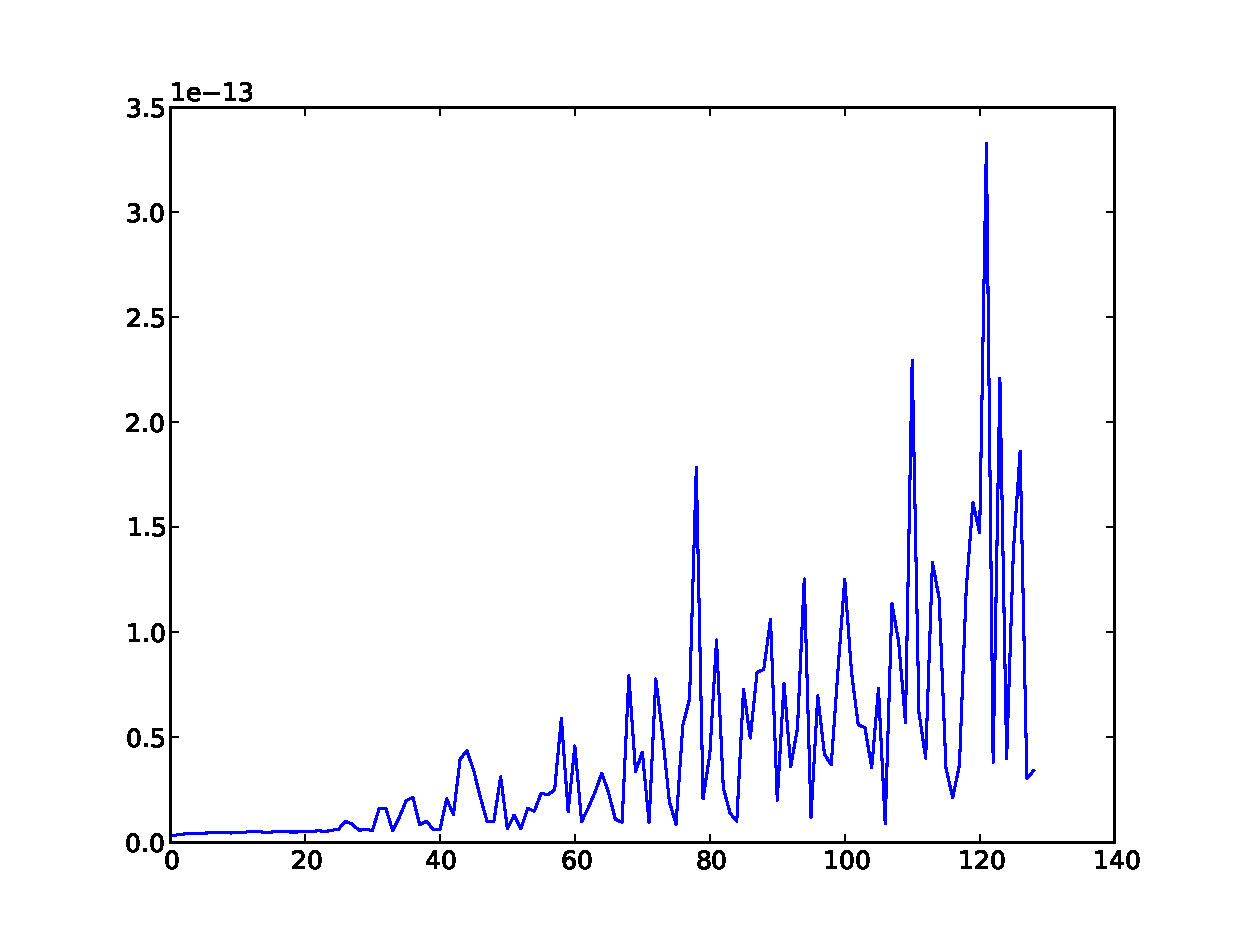
\includegraphics[width=\textwidth]{Figures/exact_numerical_2d_n130.eps}
  \caption{}
  \label{numerical_exact_FE:2D}
 \end{subfigure}
 \caption[Numerical exact error plots FE]{Error plots for the FE scheme in 1D (a) and 2D (b) when comparing with the numerical exact solution.
 Some of the terms in the numerical exact solutions are ignored to prevent overflow and these are responsible for the increasing error which is slightly larger than machine precision.}
 \label{numerical_exact_FE}
\end{figure}


\subsection{Verification of BE scheme by exact numerical solution}

The exact numerical solution to the BE scheme is found by solving the linear system which arises from the discretization (see Section \ref{theory:section:BE2D}). 
Given the $k$'th time step, the next time step is found by

\begin{align*}
 \mathbf M \mathbf u^{k+1} &= \mathbf{u}^n \\
 \mathbf{u}^{k+1} &= \mathbf{M}^{-1} \mathbf{u}^k \\
 &= \mathbf{M}^{-1}\left(\mathbf{M}^{-1} \mathbf{u}^{k-1}\right)
\end{align*}

\noindent Doing the separation to the end relates the $n$'th time step to the initial condition
\begin{equation}\label{BE_numex}
 \vec u^{k} = \left(\mathbf M^{-1}\right)^{k} \vec u^0,
\end{equation}

\noindent where $\left(\mathbf M^{-1}\right)^{k}$ is the inverse of $\mathbf M$ to the $k$'th power.\\

\noindent Taking the inverse of $\mathbf M$ will result in a dense matrix where a lot of the entries are close to zero (e.g. $10^{-20}$). 
Doing calculations with such a matrix results in a lot of round-off errors which will reduce the accuracy of the numerical exact solution. 
The error should theoretically be machine precision, but is expected to at least, be much smaller than $\Delta t$. 
Errors from both 1D and 2D simulations are shown in Figure \ref{numex:BE_errorplot}. 
Though computationally intensive, the numerical exact solution for the BE scheme has none of the limitations that were found for the FE scheme. 

\begin{figure}[H]
 \centering
 \begin{subfigure}{0.49\textwidth}
 \includegraphics[width=\textwidth]{../results/experiment_14042014_0759_BE1D_numerical_exact/results/numerical_exact.eps}
 \caption{}
\end{subfigure}
\begin{subfigure}{0.49\textwidth}
 \includegraphics[width=\textwidth]{../results/experiment_30042014_0914_BE2D_numex/results/numerical_exact.eps}
 \caption{}
\end{subfigure}
 \caption[Numerical exact error plots for BE scheme]{Plots showing the error for the BE scheme in 1D (a) and 2D (b) compared to the numerical exact solution. 
 The error is not machine precision, but significantly smaller than $\Delta t$ which for these simulations is $\Delta t=0.01$. 
 This increased error originates in the many round-off errors in the inverted matrix where a lot of terms are of the order $10^{-16}$ and smaller.}
 \label{numex:BE_errorplot}
\end{figure}

\section{Verification of the RW solver}

The aim of this section is to verify that the implemented RW model will solve the diffusion equation on the correct time scale, and to verify that the error term from the RW solver is dependent on the conversion factor, $Hc$. 
In order to carry out the tests, a new initial condition that can easily be recreated by random walkers will be introduced.
\begin{equation}
 u(t=0,x) = H\left(x-\frac{1}{2}\right)
\end{equation}
\noindent Where $H(x)$ denotes the Heaviside step function \cite{abramowitz2012handbook}, which is defined by its properties
\begin{equation}\label{Heaviside_def}
 H(x-a) = \begin{cases}
           1\;\;x > a\\
           \frac{1}{2}\;\; x = a\\ 
           0\;\;x < a
          \end{cases}
\end{equation}

\noindent The new initial condition gives a new exact solution which is found by separation of variables and Fourier series as 
\begin{equation}
 u(x,t) = \frac{1}{2} + 2\sum\limits_{n= \text{odd}}^\infty \frac{(-1)^{\frac{n-1}{2}}}{n\pi}e^{-(n\pi)^2t}\cos(n\pi x)
\end{equation}

\noindent Figure \ref{ConvergenceTestRW:Hc} verifies that the error term improves by adding more walkers. And Figure \ref{ConvergenceTestRW:dt} shows that the RW model will fulfill the chosen time step on the PDE level. 
The convergence rate is not very good, but this is expected. 
Stochastic effects causes the error to fluctuate around a certain value rather than converge to zero, making it very difficult to get a good error measure.

\begin{figure}[h]
 \centering
\begin{subfigure}[t]{0.49\textwidth}
 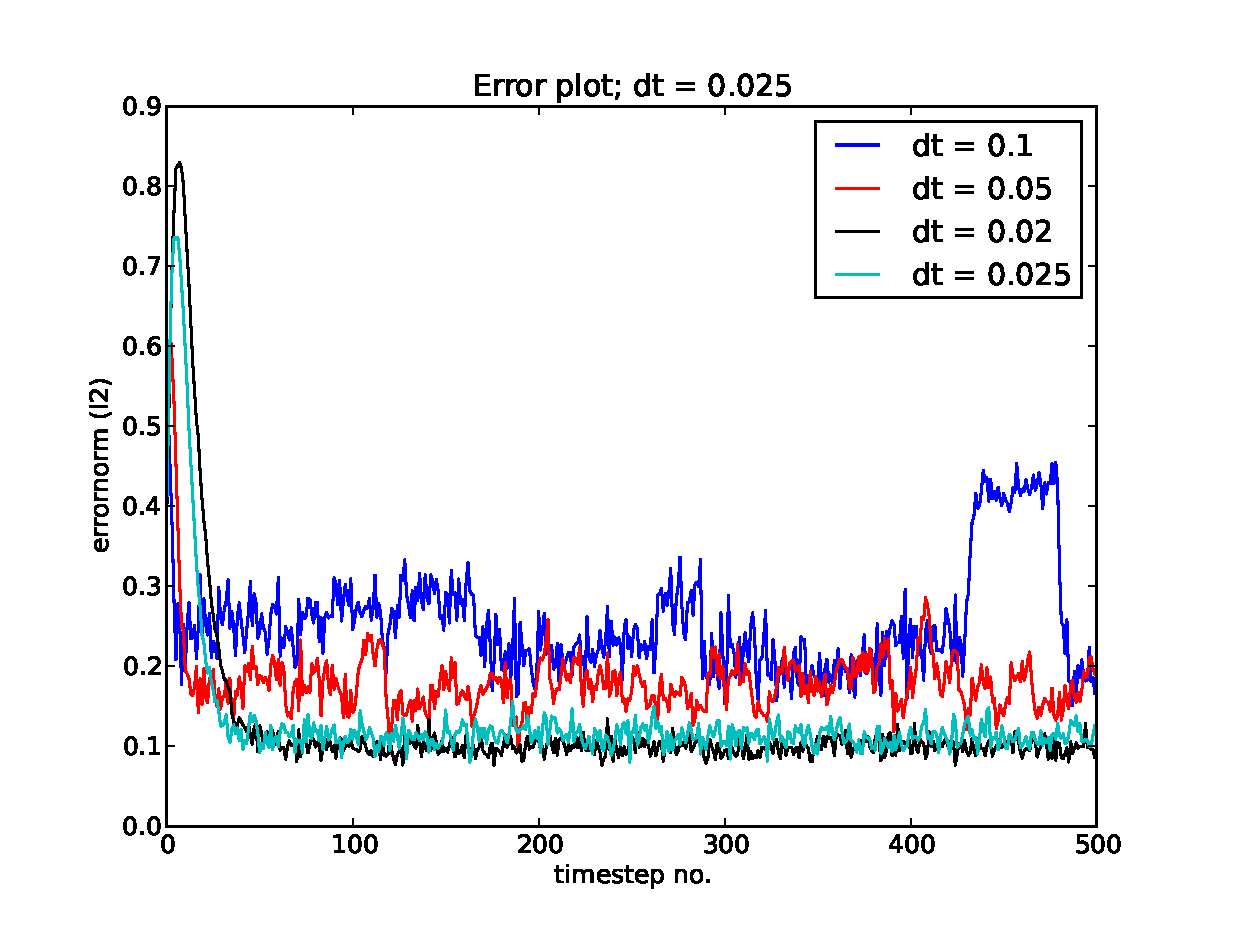
\includegraphics[width=\textwidth]{../results/experiment_01052014_1615_Redoing_RW_tests/results/errorplot.eps}
 \caption{}
 \label{ConvergenceTestRW:dt:errorplot}
\end{subfigure}
 \begin{subfigure}[t]{0.49\textwidth}
 \includegraphics[width=\textwidth]{../results/experiment_01052014_1615_Redoing_RW_tests/results/ConvergenceTest.eps}
  \caption{}
 \label{ConvergenceTestRW:dt:convergence}
\end{subfigure}
\caption[]{Error plot (a) and convergence test (b) for 1D RW solver using a Heaviside step function as initial condition. In these tests both the time step and the conversion factor are changed for each simulation, and the conversion factor follows the previously proposed limit $Hc\geq\frac{1}{\Delta t^2}$. For each $\Delta t$ the RW simulation does 250 steps with a step length calculated from \eqref{theory:step_length}. The expected convergence rate is $0.5$, and to some extent this is achieved here. Note, however, that due to fluctuations in the solution, getting a good error measure is difficult and beyond our control.}
 \label{ConvergenceTestRW:dt}
\end{figure}
% \begin{figure}[h]
%  \centering
%  \includegraphics[scale=0.4]{Figures/unit_step.eps}
%  \caption{Heaviside step function}
%  \label{heaviside}
% \end{figure}
\begin{figure}[h]
 \centering
 \begin{subfigure}[t]{0.48\textwidth}
  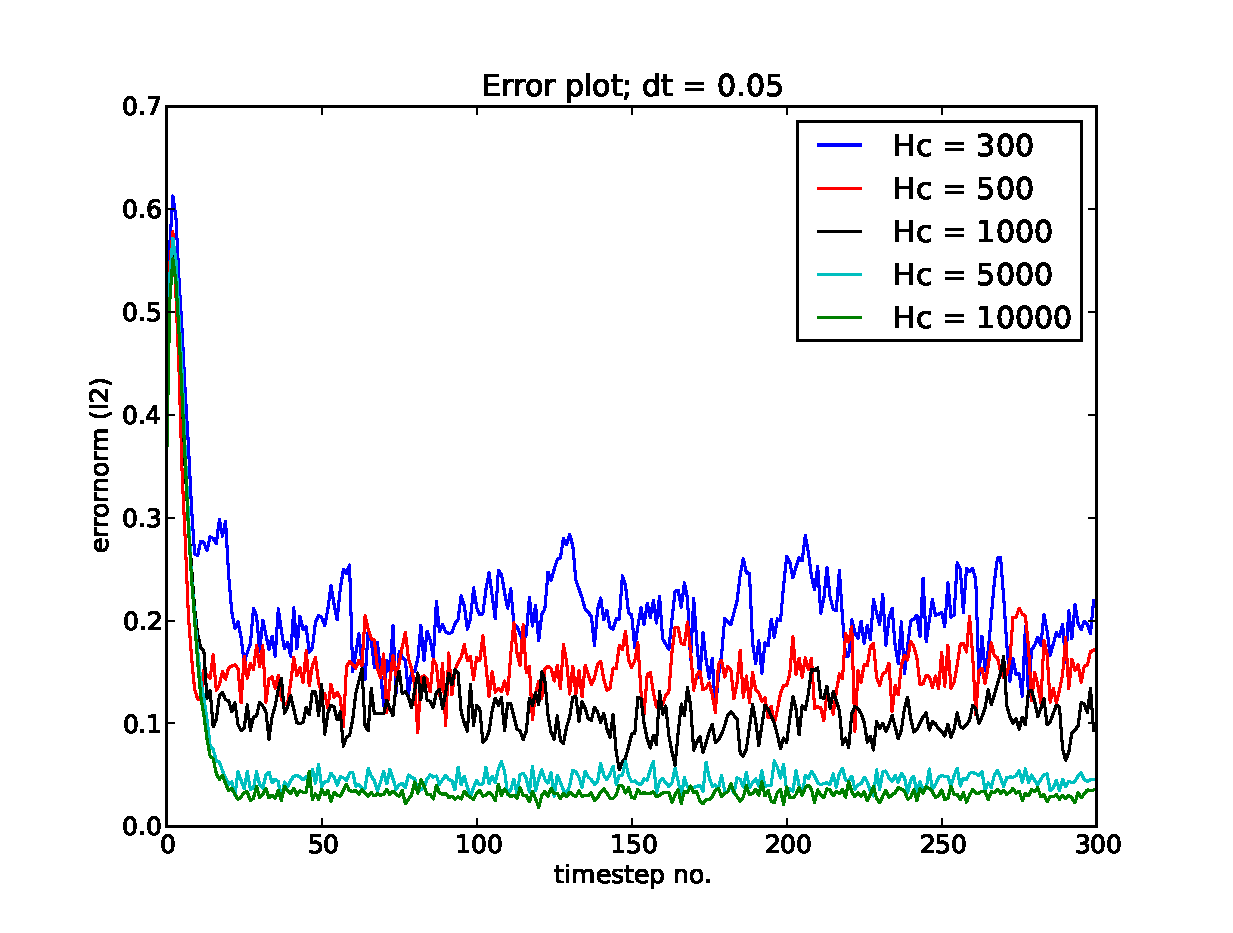
\includegraphics[width=\textwidth]{../results/experiment_02052014_0747_Redoing_RW_tests_Hc/results/errorplot.eps}
 \end{subfigure}
\begin{subfigure}[t]{0.48\textwidth}
 \includegraphics[width=\textwidth]{../results/experiment_02052014_0747_Redoing_RW_tests_Hc/results/ConvergenceTest.eps}
\end{subfigure}
\caption[Test RW]{As a comparison to Figure \ref{ConvergenceTestRW:dt}, this test has been done for the same 1D Heaviside step function as initial condition, but keeps the time step fixed at $\Delta t = 0.05$ and increases the conversion factor. The convergence rate (fig. b) is worse than for the time convergence test, and seems to reach a limit where increasing the number of walkers has little effect on the error.}
\label{ConvergenceTestRW:Hc}
\end{figure}
\clearpage

\section{Verification of the hybrid solver}
\noindent This section aims to achieve first order convergence in time for the hybrid solver by introducing a sufficient number of walkers. 
Effects of varying the number of mesh points affected by the RW solver will also be illustrated. \\

The hybrid diffusion solver is a combination of the PDE and RW solvers, which means that the error term for the hybrid model is described by 
\begin{equation}\label{analysis:hybrid_errorterm}
 \epsilon(t) = C_t \Delta t + C_x \Delta x^2 + \frac{C_{RW}}{\sqrt{Hc}},
\end{equation}
where $C_{RW}$ is an unknown stochastic coefficient.\\

\noindent From \eqref{analysis:hybrid_errorterm} it is clear that the error term from the RW solver is dominant, as it is of order $r=0.5$. 
In order to achieve first order convergence, a limitation must be placed on the conversion rate. 
Assuming that the spatial error term is negligible: 

\begin{align}
 \epsilon(t) &= C_t \Delta t + \underbrace{C_x \Delta x^2}_{\approx 0} + \frac{C_{RW}}{\sqrt{Hc}}\\
 \mathcal O(\Delta t) &\approx C_t \Delta t + \frac{C_{RW}}{\sqrt{Hc}} \\
 &\implies  \frac{1}{\sqrt{Hc}} \leq \Delta t.
\end{align}
Which finally gives the restriction on the conversion rate
\begin{equation}\label{analysis:Hc_limitation}
 Hc\geq\frac{1}{\Delta t^2}.
\end{equation}

\noindent By \eqref{analysis:Hc_limitation} the time step should be as large as possible in order to limit the number of walkers and achieve a reasonable computational performance. 
The FE scheme has a strict limitation on the time step from the stability criterion, making the BE scheme desirable. 
For this reason all tests will be done with the BE scheme. \\
Figure \ref{combined_BE1d} shows first order convergence for the hybrid model.

\begin{figure}[H]
 \centering
 \begin{subfigure}[b]{0.48\textwidth}
 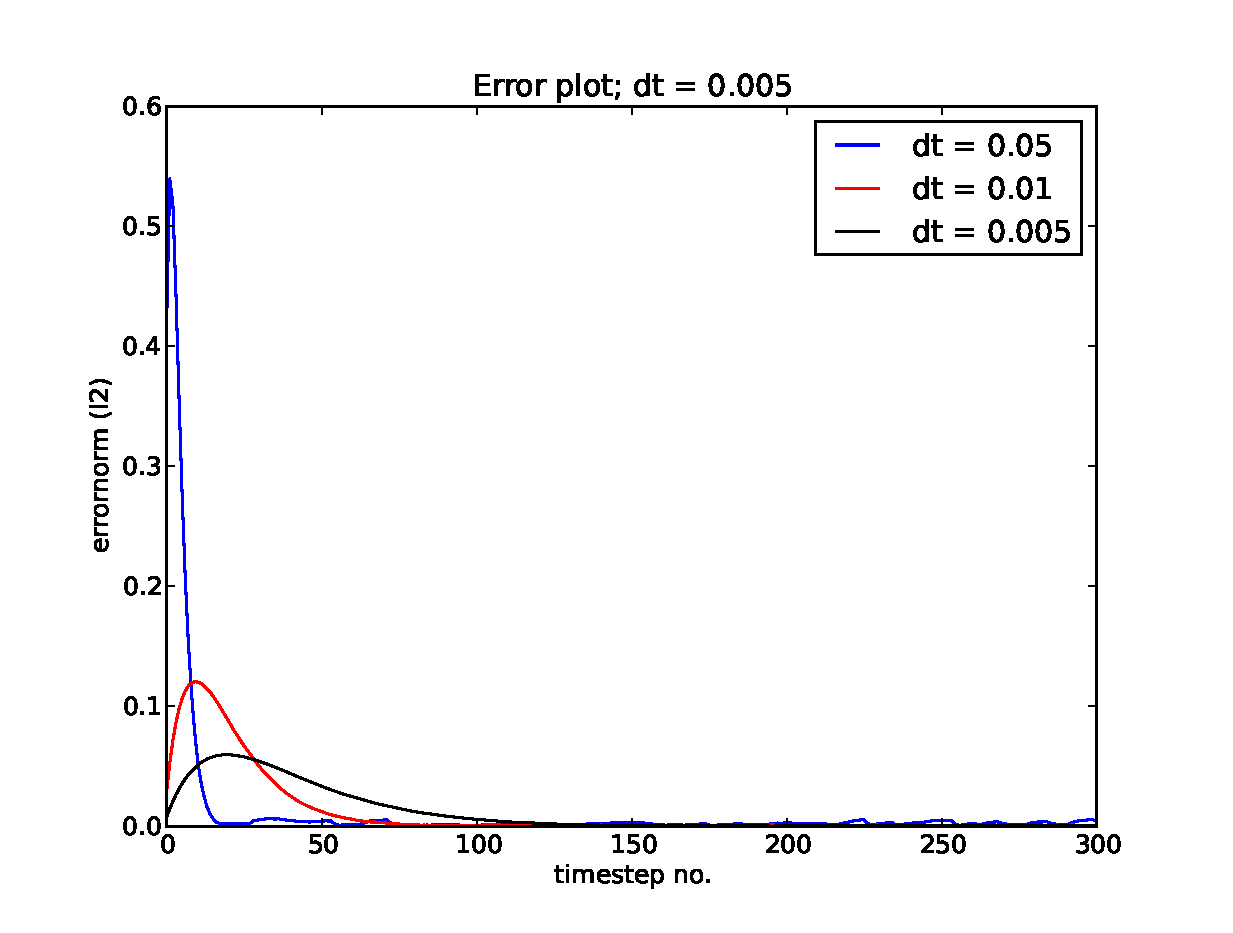
\includegraphics[width=\textwidth]{../results/experiment_15042014_0608_convergence_tests_etc/results/errorplot.eps}
\caption{}  
 \label{combined_BE1d:errorplot}
 \end{subfigure}
 \begin{subfigure}[b]{0.48\textwidth}
  \includegraphics[width=\textwidth]{../results/experiment_15042014_0608_convergence_tests_etc/results/ConvergenceTest.eps}
  \caption{}
   \label{combined_BE1d:convergence}
 \end{subfigure}
 \caption[Error test for BE combined with RW in 1D]{\ref{combined_BE1d:errorplot} shows the error plot for a test where $\Delta x$ was fixed at $\Delta x = \frac{1}{100}$ and $\Delta t$ was reduced from $0.05$ to $0.01$ and finally to $0.005$. 
 The conversion rate, $Hc$ was updated for each simulation to have the value $Hc = \frac{1}{\Delta t^2}$, meaning the error from the walkers should be smaller than the error from the time derivative. 
 Walkers are placed on 10\% of the mesh from $x=0.4$ to $x=0.5$. 
 \ref{combined_BE1d:convergence} shows the convergence rate in time for the same test.}
 \label{combined_BE1d}
\end{figure}

Decreasing or increasing the relative size of the microscopic model has serious effects on the error. This is illustrated in Figure \ref{testing_walk_area_size_BE}

\begin{figure}[H]
\centering
\begin{subfigure}[b]{0.48\textwidth}
 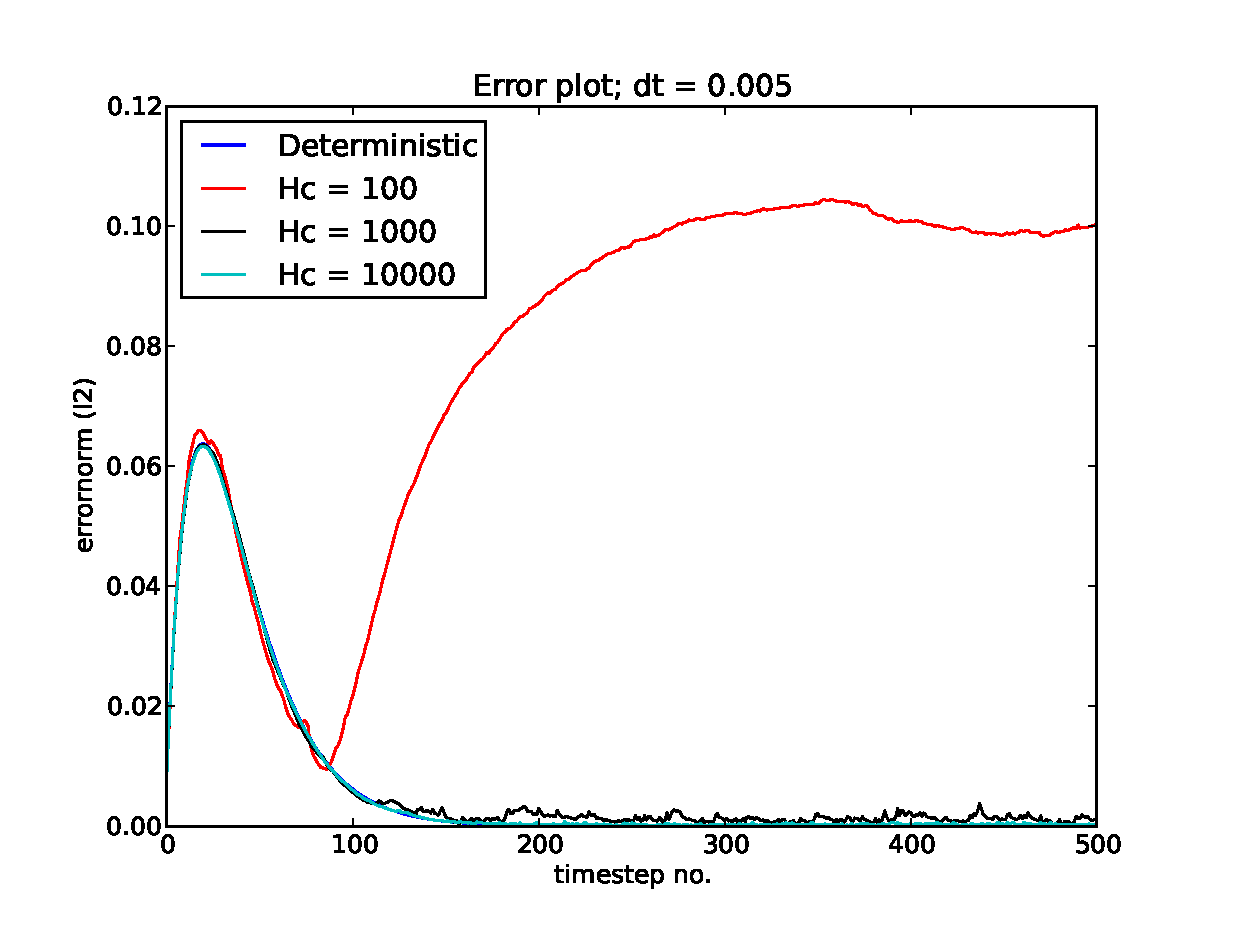
\includegraphics[width=\textwidth]{../results/experiment_16042014_1139_convergence_tests_etc/results/errorplot.eps}
 \caption{Walkers on 5\% of the mesh points.}
 \label{errorplot_BE1D_walk_5_percent}
\end{subfigure}
\begin{subfigure}[b]{0.48\textwidth}
 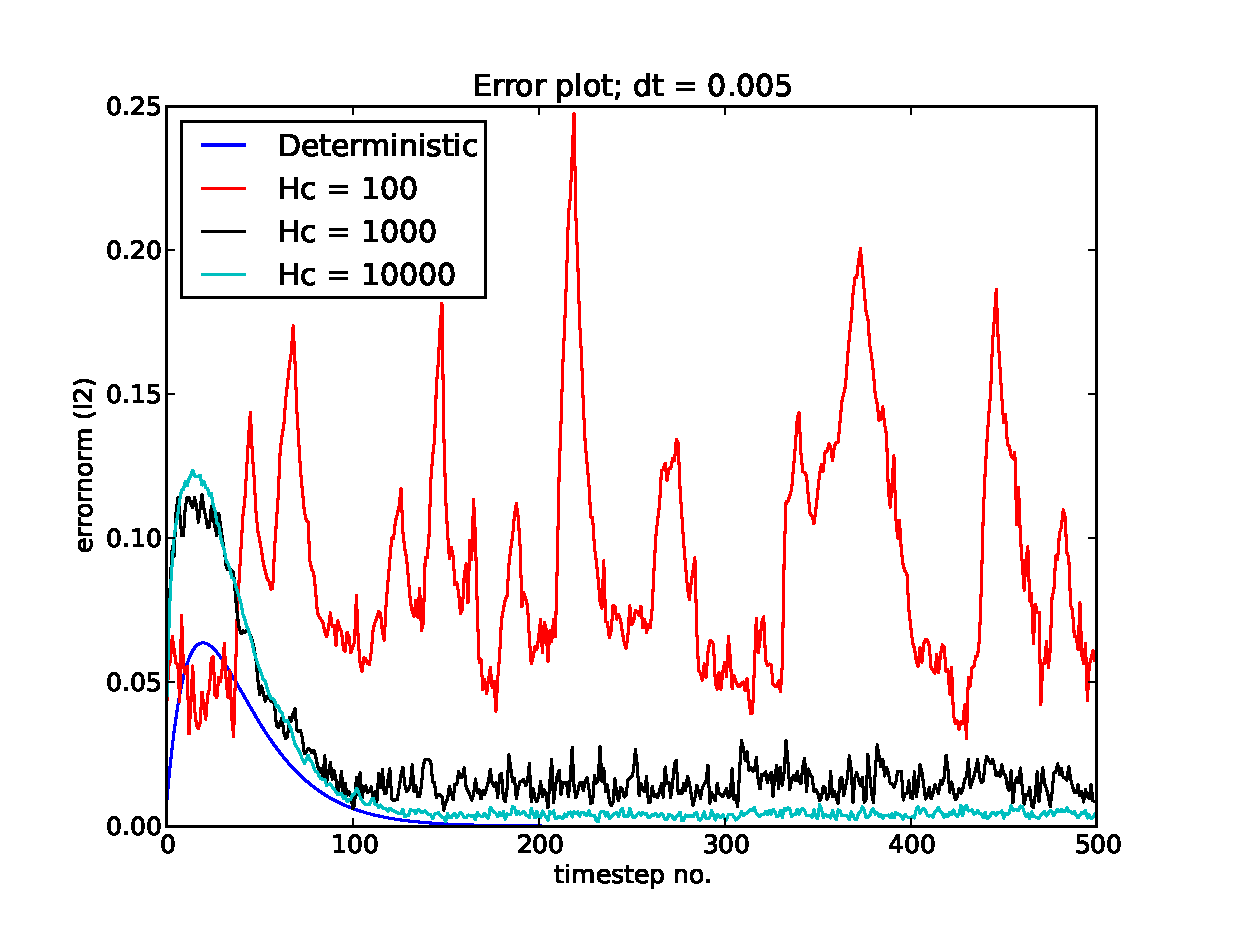
\includegraphics[width=\textwidth]{../results/experiment_16042014_1202_tests_35percent_walkers/results/errorplot.eps}
 \caption{Walkers on 35\% of the mesh points.}
 \label{errorplot_BE1D_walk_35_percent}
\end{subfigure}
\caption[Effects of increasing relative size of walk area]{The effect of increasing the size of the walk area for a fixed $\Delta t = 0.05$ and $\Delta x = 0.01$ using the BE discretization.}
\label{testing_walk_area_size_BE}
\end{figure}